
\lecture{Introduction to Discrete}{introduction-to-discrete-data}
\section{Introduction to Discrete Data}

\title{Introduction to Discrete Data}
\subtitle{Quantitative Data}

%\author{Kelly Black}
%\institute{Clarkson University}
\date{6 February 2013}

\begin{frame}
  \titlepage
\end{frame}

\begin{frame}
  \frametitle{Outline}
  \tableofcontents[hideothersubsections,sectionstyle=show/hide]
\end{frame}


\iftoggle{clicker}{%
  \subsection{Clicker Quiz}
  \begin{frame}
    \frametitle{Clicker Quiz}

    The number of items produced per hour in a given factor is normally
    distributed with a mean of 230 items per hour and a standard
    deviation of 25 items per hour. What is the probability that in a
    given time period there will be more than 260 items per hour?

    \begin{tabular}{l@{\hspace{3em}}l@{\hspace{3em}}l@{\hspace{3em}}l}
      A:  0.0 & B: 0.1151  & C: 0.8849  & D: 1.20
    \end{tabular}


  \end{frame}
}





\subsection{Qualitative Data}

\begin{frame}{Qualitative Data}

  \begin{definition}{Discrete Data}

    A discrete random variable produces a countable number of
    values. The values are one of a fixed set of values.
    
  \end{definition}

  \begin{definition}{Continuous Data}

    The numbers produced come from an infinite number of possible
    outcomes.
    
  \end{definition}

  
\end{frame}


\begin{frame}{Discrete Data Examples}

  \begin{itemize}
  \item Someone reads an article, and we ask them to rate it on a
    scale from one to five.

  \item We give a person three different soft drinks and ask them to
    tell us which one they like the best.

  \item We count the number of complaints that a department in a
    business receives over a preset period of time.

  \end{itemize}
  
\end{frame}

\subsection{Example}

\begin{frame}{The Data - An example}

  The people coming into a local drug store are monitored to see where
  people go to make a purchase. The following data is found: \\
  \begin{tabular}{l}
    Health Care \\
    Health Care \\
    Photo \\
    Candy \\
    Health Care \\
    Cosmetics \\
    Health Care \\
    Candy \\
    Health Care \\
    Cosmetics \\
    Cosmetics \\
    Health Care \\
    Photo 
  \end{tabular}

  How do we analyze this?
  
\end{frame}


\subsection{Frequency}

\begin{frame}{Frequencies}

  One way is to count the number of occurrences: \\
  \only<1>
  {
    \begin{tabular}{l}
      Health Care \\
      Health Care \\
      Photo \\
      Candy \\
      Health Care \\
      Cosmetics \\
      Health Care \\
      Candy \\
      Health Care \\
      Cosmetics \\
      Cosmetics \\
      Health Care \\
      Photo 
    \end{tabular}
  }


  \only<2>
  {
    \begin{tabular}{l|l}
      Department  & Frequency \\ \hline
      Health Care & 6 \\
      Photo       & 2 \\
      Candy       & 2 \\
      Cosmetics   & 3 \\
    \end{tabular}
  }


  \only<3>
  {
    \begin{tabular}{l|l}
      Department  & Relative Frequency \\ \hline
      Health Care & 6/13 \\
      Photo       & 2/13 \\
      Candy       & 2/13 \\
      Cosmetics   & 3/13 \\
    \end{tabular}
  }

  
\end{frame}


\subsection{Graphical Views of Discrete Data}

\begin{frame}{Graphical Views of the Data}

  The data can be viewed as a bar plot.

  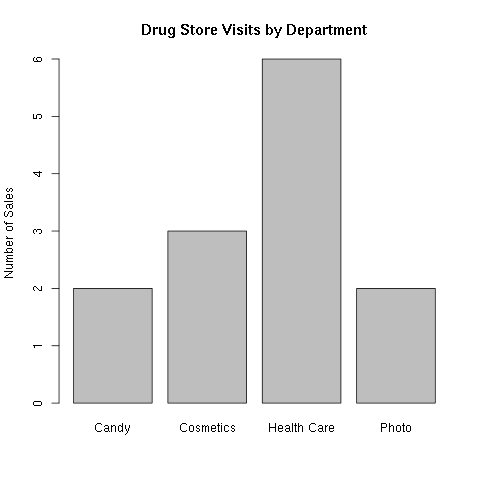
\includegraphics[width=6cm]{img/drugStoreBarPlot}
  
\end{frame}

\begin{frame}{Graphical Views of the Data}

  The data can be viewed as a Pareto plot.

  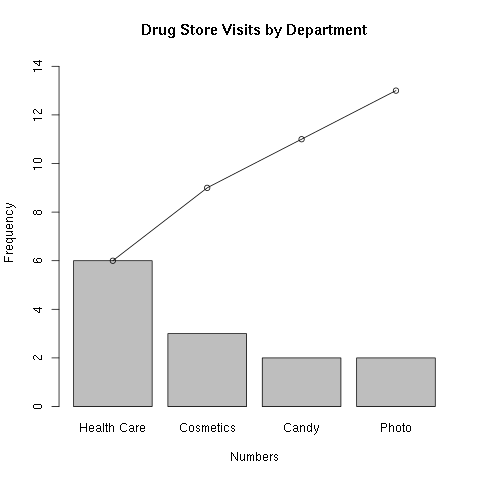
\includegraphics[width=6cm]{img/drugStorePareto}
  
\end{frame}


\iftoggle{clicker}{%
  \begin{frame}
    \frametitle{Clicker Quiz}

    Which plot below represents the Pareto chart for the following data:

    A, A, C, B, B, B, D

    \begin{tabular}{ccc}
      A: 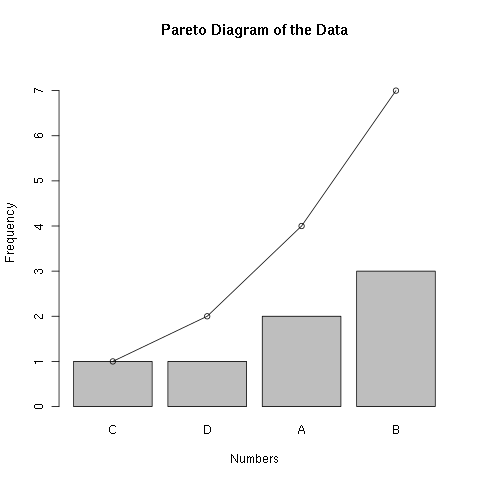
\includegraphics[width=3cm]{img/paretoQuizW1D2-a} &
      B: 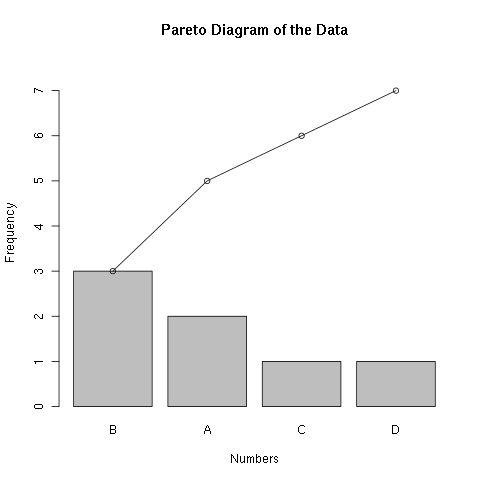
\includegraphics[width=3cm]{img/paretoQuizW1D2-b} &
      C: 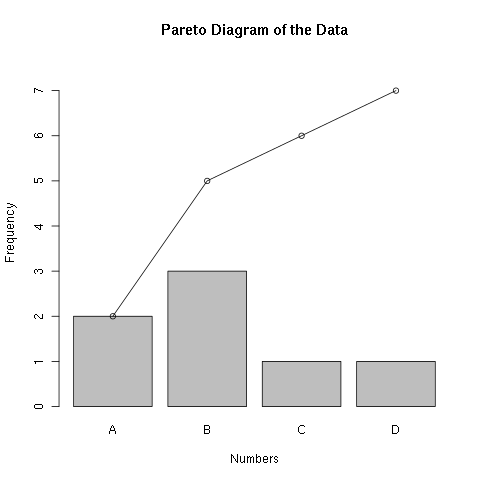
\includegraphics[width=3cm]{img/paretoQuizW1D2-c}
    \end{tabular}

  \end{frame}
}


\begin{frame}
  \frametitle{Cross Tabular Tables}


  \begin{columns}
    \column{.15\textwidth}

    \begin{tabular}{ll}
      $Q_{1}$ & $Q_{2}$ \\ \hline
      A & Y \\
      B & Y \\
      B & N \\
      B & N \\
      A & N \\
      A & N \\
      B & N
    \end{tabular}

    \column{.85\textwidth}

    \only<2->
    {
      \begin{tabular}{l|l|l|l}
        $Q_1 \backslash Q_2$ & Y & N & Row Total \\
        A & 1 & 2 & 3 \\ \hline
        B & 1 & 3 & 4 \\ \hline
        Col. Total & 2 & 5 & 7
      \end{tabular}
    }

    \vfill

    \only<3>
    {
      {\color{red}{Relative frequency}}
      \begin{tabular}{l|l|l|l}
        $Q_1 \backslash Q_2$ & Y & N & Row Total \\
        A & 0.14 & 0.29 & 0.43 \\ \hline
        B & 0.14 & 0.43 & 0.57 \\ \hline
        Col. Total & 0.29 & 0.71 & 1.0
      \end{tabular}
    }

    \only<4>
    {
      {\color{red}{Marginal Distribution by Rows}}
      \begin{tabular}{l|l|l|l}
        $Q_1 \backslash Q_2$ & Row Total & Relative Frequency\\
        $Q_1 \backslash Q_2$ & Y & N & Row Total \\
        A & 0.33 & 0.67 & 1.0 \\ \hline
        B & 0.25 & 0.75 & 1.0 \\ \hline
        Col. Total & 0.0.29 & 0.71 & 1.0
      \end{tabular}
    }

    \only<5>
    {
      {\color{red}{Marginal Distribution by Columns}}
      \begin{tabular}{l|l|l|l}
        $Q_1 \backslash Q_2$ & Y & N & Row Total \\
        A & 0.50 & 0.40 & 0.43 \\ \hline
        B & 0.50 & 0.60 & 0.57 \\ \hline
        Col. Total & 1 & 1 & 1
      \end{tabular}
    }

  \end{columns}

\end{frame}


\iftoggle{clicker}{%
  \begin{frame}
    \frametitle{Clicker Quiz}


    Determine the table for this data with the row percentages (Marginal Distribution by Rows):

    \begin{columns}
      \column{.25\textwidth}

      \begin{tabular}{l|l}
        $Q_{1}$ & $Q_{2}$ \\ \hline
        a & d \\
        a & e \\
        b & e \\
        a & d \\
        b & e \\
        a & d
      \end{tabular}


      \column{.75\textwidth}

      1:
      \begin{tabular}{l|l|l|l}
        $Q_1 \backslash Q_2$ & d & e & Row \\
        a & 3/4 & 1/4 & 1.0 \\ \hline
        b & 0.0 & 1.0 & 1.0 \\ \hline
        Col.  & 3/6 & 3/6 & 1.0
      \end{tabular}

      \rule{5cm}{0.05cm}

      2:
      \begin{tabular}{l|l|l|l}
        $Q_1 \backslash Q_2$ & d & e & Row  \\
        a & 1.0 & 1/3 & 4/6 \\ \hline
        b & 0.0 & 2/3 & 2/6 \\ \hline
        Col.  & 1.0 & 1.0 & 1.0
      \end{tabular}

      \rule{5cm}{0.05cm}

      3:
      \begin{tabular}{l|l|l|l}
        $Q_1 \backslash Q_2$ & d & e & Row  \\
        a & 1.0 & 0.0 & 1.0 \\ \hline
        b & 1/3 & 2/3 & 1.0 \\ \hline
        Col.  & 3/5 & 2/5 & 1.0
      \end{tabular}


    \end{columns}

  \end{frame}
}


\begin{frame}{Pie Charts}

  Pie charts are the work of the devil. People who use them are the
  kind of people who have poor personal hygiene. 

  \vfill

  \centerline{
\includegraphics[width=4cm]{img/grumpyPieChart}}

  %\tiny{Just say'n}
  
\end{frame}

% LocalWords:  Clarkson pausesection hideallsubsections Bivariate
